
\section{Statement of Work (SOW)}
The project's aim is to develop a minaturized high-sensitivity, low-noise magnetic gradiometer. Our approach is to mimic the mechanism found in magnetosomes, the specialized cells four from bacteria to higher vertebrates such as fish and birds (see \ref{sec:inno}). This is comprised of four main tasks: modeling and simulation, microfabrication process design, circuit design, and device manufacture and testing. Each Phase (I,II,III) will include these four tasks.
\subsection{Phase I}
\subsubsection{Modeling and simulation}
\begin{itemize}
\item A general description of the objective (for each defined task/activity)
\item A detailed description of the approach to be taken to accomplish each defined task/activity
\item Identification of the primary organization responsible for task execution (prime, sub, team member, by name, etc.)
\item The completion criteria for each task/activity - a product, event or milestone that defines its completion
\item Define all deliverables (reporting, data, reports, software, etc.) to be provided to the Government in support of the proposed research tasks/activities
\item Identify whether government-furnished equipment is requested and, if so, the required quantity and delivery schedule
\item Clearly identify any Risk Reduction tasks AND
\item Clearly identify any tasks/subtasks (prime or subcontracted) that will be accomplished on-campus at a university.
Note: Each program phase must be separately defined in the SOW. Include a SOW for each
subcontractor and/or consultant in the Cost Proposal Volume. Do not include any proprietary
information in the SOW(s).
\end{itemize}
\subsubsection{Microfabrication}
\subsubsection{Circuit design}
\subsubsection{Manufacture and testing}
\subsection{Phase II}
\subsubsection{Modeling and simulation}
\subsubsection{Microfabrication}
\subsubsection{Circuit design}
\subsubsection{Manufacture and testing}
\subsection{Phase III}
\subsubsection{Modeling and simulation}
\subsubsection{Microfabrication}
\subsubsection{Circuit design}
\subsubsection{Manufacture and testing}

\section{Innovative Claims}\label{sec:inno}

Our approach is to design a sensor based on a magnetoreceptive mechanism used in nature - magnetite crystals torqued by external magnetic fields open ion channels in the cell wall. To mimic this, we propose a microfabricated MEMS sensor, with a layer of magnetic material on top of piezo electric cantilevers. When forced with an exernal field, torque induced on the magnet create stress in the piezo, and thus a voltage is produced. There are three advantages to this approach. First, microfabrication allows for a small size. Second, by orienting individual sensing elements in anti-series order, the output is natively a gradiometer. Third, by selecting the resonant frequency of the cantilever carefully, we can create a gradiometer which outputs a spectrogram directly. Though fluxgates can be microfabricated and function as gradiometers, they suffer a size/sensitivity tradeoff. Microfabricated atmonic magnetometers are sensitive but don't function natively as gradiometers. Other micro-scale magnetometers, namely Lorentz-type, which operate on a similar mechanism, are not yet sensitive enough and haven't been used as frequency-domain gradiometers, as in the proposed design.

\section{Detailed Technical Approach}

Magnetometers serve an important role in investigating biologically generated electromagnetic fields, such as those created by neuronal currents, or geological magnetic fields. Typically, magnetometers are unable to achieve high sensitivity in an ambient, unshielded environment - getting to femtotesla level sensitivity requires magnetic shield and cryogenic sensors, such as SQUID \cite{lenz2006magnetic}. The novel spin relaxation free magnetometer has been minaturized and achieves less than 10 fT/$\sqrt{Hz}$, but still requires shielding and lacks directional sensitivity \cite{shah2013compact}. Fluxgates have achieved pT level resolution at small size, but this is insufficient for biomagnetic field measurement \cite{sasada2002orthogonal,uchiyama2014highly,sasada2014fundamental} 

\begin{figure}[h]
  \centering
  \begin{subfigure}
    \centering
    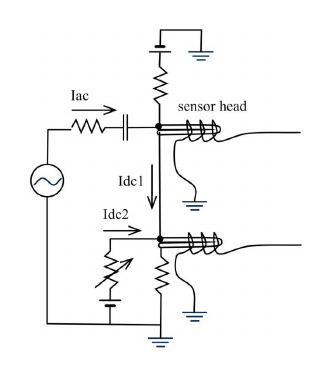
\includegraphics[width=0.5\textwidth]{fmofg}
  \end{subfigure}
  \begin{subfigure}
    \centering
    
\includegraphics[width=0.5\textwidth]{fmofg2}
  \end{subfigure}
\caption{Fundamental-mode orthogonal fluxgate gradiometer \cite{sasada2014fundamental}.}
\label{fig:fmofg}
\end{figure}
Lorenz-type magnetometers (which translate magnetic fields into mechanical actuation of a magnet or current carrying wire) have been built in MEMS substrates, but are as yet insufficiently sensitive and require shielding \cite{sinha201627,kyynarainen20083d,kumar2015ultra,thompson2009parametrically}

\begin{figure}[h]
\centering
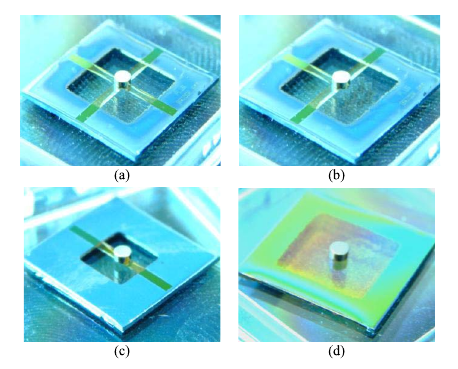
\includegraphics[width=0.5\textwidth]{lorenz}
\caption{Lorenz-type magnetometer \cite{sinha201627}.}
\label{fig:nd_lorenz}
\end{figure}

\begin{figure}[h]
\centering
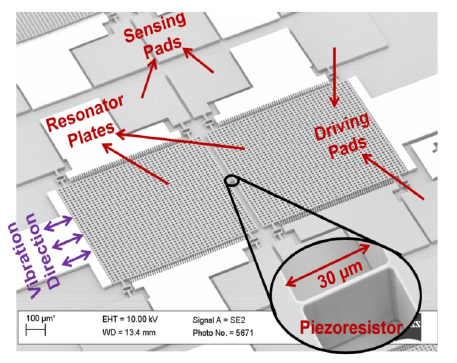
\includegraphics[width=0.5\textwidth]{lorenz2}
\caption{Lorenz-type magnetometer \cite{kumar2015ultra}.}
\label{fig:lorenz}
\end{figure}

In nature, many organisms have a sense of magnetoreception used for navigation, from magnetotactic bacteria to birds. Two mechanisms have been proposed: a spin-selective (and thus field-sensitive) chemical reaction rate, or magnetite crystals which are actuated by external fields and activate ion channels in the cell membrane \cite{johnsen2005physics,dodson2013radical,kirschvink2001magnetite}. Mesurements of these magnetosomes show a magnetic dipole moment of up to 100fA/m$^2$ \cite{hanzlik2002pulsed,eder2012magnetic}.

\begin{figure}
\centering
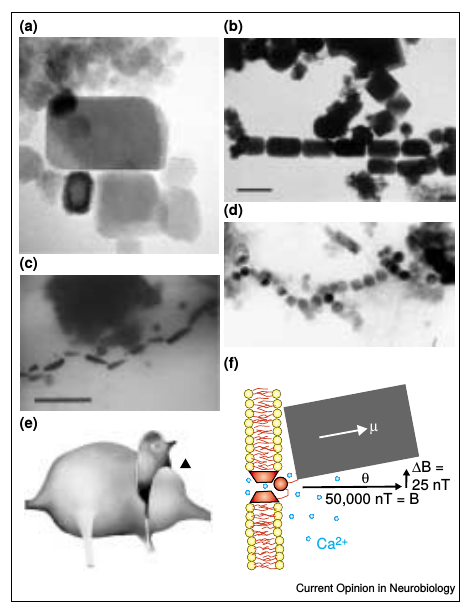
\includegraphics[width=0.5\textwidth]{kirsh2001}
\caption{Magnetosomal mechanism \cite{kirschvink2001magnetite}.}
\label{fig:magnetsosome}
\end{figure}

Our approach is to mimic the approach found in magnetosomes, with some key modifications so that is frequency-selective and functions inherently as a gradiometer and thus does not require shielding. The closest biomimetic sensor is a flow sensor which uses ferromagnetic cilia to detect microfluidic flow rates \cite{alfadhel2014magnetic}.

\begin{figure}[h]
\centering
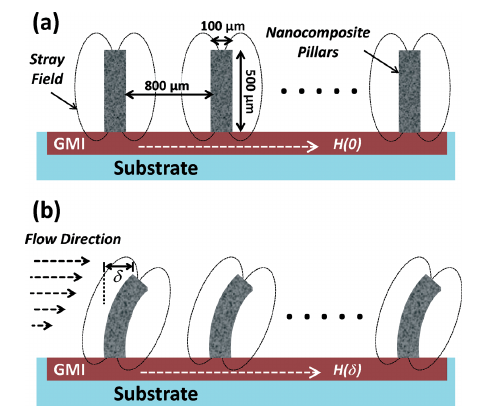
\includegraphics[width=0.5\textwidth]{cilia}
\caption{Magnetic cilia flow sensor \cite{alfadhel2014magnetic}.}
\label{fig:cilia}
\end{figure}

To acomplish this, we propose layering single-domain magnetic crystals on top of piezoelectric cantilevers. The moment induced on the magnetic layer is:

\begin{equation}
  M=\vec{\mu} \times \vec{B}
\end{equation}

which induces stress in the cantilever, and the piezoelectric effect generates a voltage. Two features are possible from the cantilever design: frequency selection and grdiometery. As in \cite{shen2008design}, a cantilever has a resonant frequency, which can be modifying through geometrical parameters. Peak response will be achieved at this frequency. By selection many cantilevers of different dimensions, each corresponding to a separate output, the magnetometer output is a spectrometer. Many cantilevers at the same resonance in series generate a largeer voltage; in anti-series, the difference is taken, thus functioning as a gradiometer with very high spatial resolution. 

Even though biological magnetoreception is limited to nT sensitivity, our design will allow us to surpass this. First, by careful selection of materials (such as Co-Pt or rare-earth magnets) \cite{coey2010magnetism, arnold2009permanent} we can have much higher magnetic dipole moment, and thus higher moment. Second, by careful selection of geometery, we can employ parametric resonance \cite{van2006resonant}. Finally, using two banks of cantilevers in series in anti-series, we both boost the voltage and create a high resolution gradiometer.


\cite{levinzon2004fundamental} Fundamental noise limit of piezoelectric accelerometer

\begin{figure}
\centering
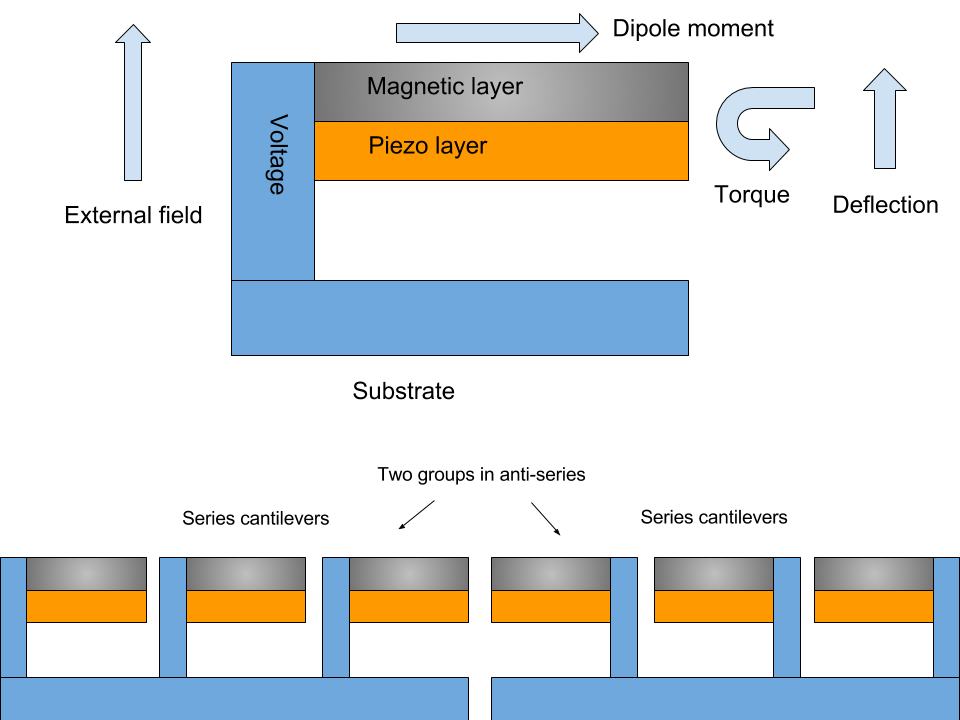
\includegraphics[width=0.75\textwidth]{biomag}
\caption{Diagram of proposed design.}
\label{fig:diagram}
\end{figure}

Fabrication methods?
Scaling
COTS
\begin{table}[h!]
\centering
  \begin{tabular}{|c||c|c|}
    \hline
    Phase & Milestone & Date\\
    \hline
    \hline
    & & \\
    \hline
    & & \\
    \hline
    & & \\
    \hline
    & & \\
    \hline
    & & \\
    \hline
  \end{tabular}
\caption{Milestones schedule}
\label{table:sched}
\end{table}

    

Phase 1: Base Period (18 months)
AMBIIENT Phase 1 will demonstrate sensor functionality and performance in a laboratory
setting meeting the performance metrics as indicated in Table 1. The sensor volume requirements
are relaxed in Phase 1 to allow independent development of components and/or use of COTS
components for initial proof of concept. The power metric reflects the total consumption of all
sensor components (P=ΣVi*Ii), including all vacuum and photonic components, as well as any
necessary thermal control. Power conditioning and controlling electronics are not included in the
power consumption metric of this phase.
Phase 2: Option 1 (12 months)
AMBIIENT Phase 2 will develop and demonstrate an integrated sensor head meeting the
performance and SWaP metrics of Table 1, and including all vacuum, photonic, and thermal
control components. The sensor volume assumes a rectangular parallelepiped or cylindrical
geometry. The sensor will be sufficiently rugged and compact to allow for temperature testing as
indicated in Table 1. The performer will support transportation to and test of one sensor, along
with suitably portable control electronics, at a government testing facility as directed by
DARPA, two months prior to the conclusion of Phase 2.
Phase 3: Option 2 (12 months)
AMBIIENT Phase 3 will demonstrate a fully integrated gradiometer comprising all control
electronics, power conditioning, and packaging, meeting all performance metrics of Table 1.
Phase 3 prototype gradiometers should require only a single external power source and will
provide digital output of total field and gradient at data rates as indicated in Table 1. Power
consumption will be determined by P = V * I of the power input and volume will be separately
computed for the sensor and control modules. Five complete prototype gradiometers will be
delivered to a government testing facility, as directed by DARPA, at the conclusion of Phase 3.


This is the centerpiece of the proposal and should provide a detailed description of the
proposed technology, including analysis and modeling where available, to substantiate the
innovative claims of Section II.B.

This section must include a proposed milestone table and
performance objectives, by phase, similar to Table 1 of this BAA. Proposals should clearly
explain the technical approach that will be employed to meet or exceed each program metric
and provide ample justification as to why the approach is feasible. Where applicable, analysis
should include concise performance budget tables, e.g. for contributory error or power
budget elements.

\section{Risk Analysis and Mitigation Plan}

\begin{table}[h!]
\centering
\begin{tabular}{|c||c|c|c|}
    \hline
    Risk & Probability & Impact & Plan\\
    \hline
    \hline
    & & & \\
    \hline
    & & & \\
    \hline
    & & & \\
    \hline
    & & & \\
    \hline
    & & & \\
    \hline
\end{tabular}
\caption{Risk matrix}
\label{table:risk}
\end{table}

Identify the major technical and programmatic risks in the program. Include a risk matrix.
For each risk, assign a probability of occurrence on a scale of 1-10, where 10 indicates a high
likelihood that the risk will impact program success, as well as an assessment of impact, also
on a scale of 1-10, where 10 indicates that this risk would maximally limit the program from
delivering prototypes on schedule or meeting performance objectives. For each item with
total risk (likelihood × impact) exceeding 40, include a plan for mitigating the risk and
assessing risk reduction.
Where necessary, parallel risk reduction tasks may be proposed, e.g. concurrent development
of redundant techniques or components. The proposal must differentiate the primary
technical path from risk reduction tasks, which should be uniquely identified in the SOW and
separately costed as optional tasks in Volume II.
\section{Schedule and Milestones}
Include a high-level Gantt chart outlining major technical tasks and measureable milestones
by phase. At a minimum, the schedule should include each SOW task of Volume 1, Section
II.A. Where risk reduction tasks are proposed, the schedule should include a milestone for
assessment and removal of redundant tasks.

\section{Test Plan}
Describe how compliance with the proposed metrics and milestones will be demonstrated in
each phase of the program. The test plan should be structured so that compliant performance
can be verified prior to delivery of hardware for government test and evaluation.
\subsection{Phase I}

\subsection{Phase II}

\subsection{Phase III}

\section{Results and Technology Transfer}
Description of the results, products, transferable technology, and expected technology
transfer. This should also address mitigation of life-cycle and sustainment risks associated
with transitioning intellectual property for U.S. military applications, if applicable. See also
Section IV.B.10, “Intellectual Property.”

\section{Ongoing Research}
Comparison with other ongoing research indicating advantages and disadvantages of the
proposed effort.
\section{Proposer Accomplishments}
Discussion of proposer’s previous accomplishments and work in closely related research
areas. In this section, also include any ongoing research projects or pending proposal activity
that technically overlaps with the proposed effort, including funding source, administrative
point of contact, and the program management plan for combining and de-conflicting the
efforts.
\section{Facilities}
Description of the facilities that will be used for the proposed effort.
\section{Teaming}
Description of the formal teaming agreements that are required to execute this program.
Describe the programmatic relationship between investigators and the rationale for choosing
this teaming strategy. Present a coherent organization chart and integrated management
strategy for the program team. For each person, indicate: (1) name, (2) affiliation, (3)
abbreviated listing of all technical area tasks they will work on with roles, responsibilities,
and percent time indicated, (4) discussion of the proposers’ previous accomplishments,
relevant expertise and/or unique capabilities.
